%!TEX root = TFG.tex

%Definição
%Explicação
%Teoria 
%Ligação com o trabalho

\chapter{Literature Review}\label{literature_review}

\section{State of the Art}

    In this section similar works are cited with the goal of contextualizing our proposal, expressing relations and differences to approaches currently found in the industry and academic research. 

\subsection{Zoox: Simulation for Autonomous Driving}

    Zoox is a startup founded in 2014 with the goal of bringing autonomous mobility experiences to the market. The company is in development stage \cite{zoox-linkedin} and doesn't have widespread marketing campaigns \cite{zoox-official-website}. However, it stands out in the industry due to demonstrations of their autonomous-driving technology. 
    
    The startup made its "tech media" debut on Unreal Engine SIGGRAPH 2017 User Group \cite{zoox-unreal-siggraph-2017} with a technology sneak peek of its simulation pipeline. There they showed a car with 8 sensors as demonstrated in \autoref{fig:zoox-car-sensors} and focused on presenting an elaborate virtual environment with the goal to enhance the passenger experience using visualizations of interpretations of autonomous-driving algorithms as shown in \autoref{fig:zoox-simulation-basic-model}.
    
    \begin{figure}[H]
     \caption{\label{fig:zoox-car-sensors}
Zoox demonstration car}
     \begin{center}
        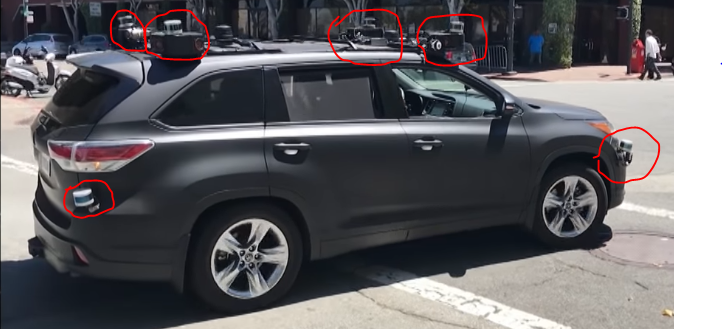
\includegraphics[width=0.8\textwidth]{images/zoox-car_red-lines.PNG}
     \end{center}
     \legend{Source: Adapted from \cite{zoox-unreal-siggraph-2017}.}
    \end{figure}
    
    \begin{figure}[H]
     \caption{\label{fig:zoox-simulation-basic-model}
Zoox simulation environment}
     \begin{center}
        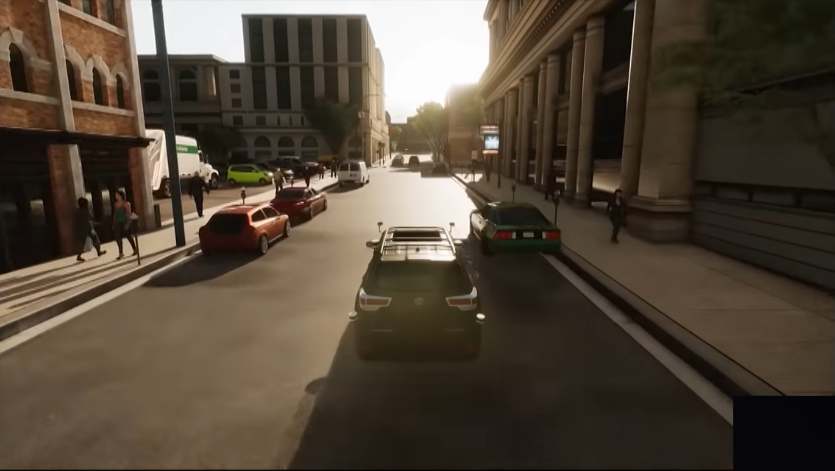
\includegraphics[width=0.8\textwidth]{images/zoox-simulation-basic-model.png}
     \end{center}
     \legend{Source: Adapted from \cite{zoox-unreal-siggraph-2017}.}
    \end{figure}

    On 2018 Zoox introduced their Youtube channel \cite{zoox-youtube-channel} with an evolved demonstration of the route network simulation from SIGGRAPH 2017, shown in \autoref{fig:zoox-siggraph-route-network}, with more entities and an instant route estimation of the autonomous-driving algorithm \cite{zoox-fully-autonomous-driving} as shown in \autoref{fig:zoox-simulation-monitoring}.
    
    \begin{figure}[H]
     \caption{\label{fig:zoox-siggraph-route-network}
Zoox route network}
     \begin{center}
        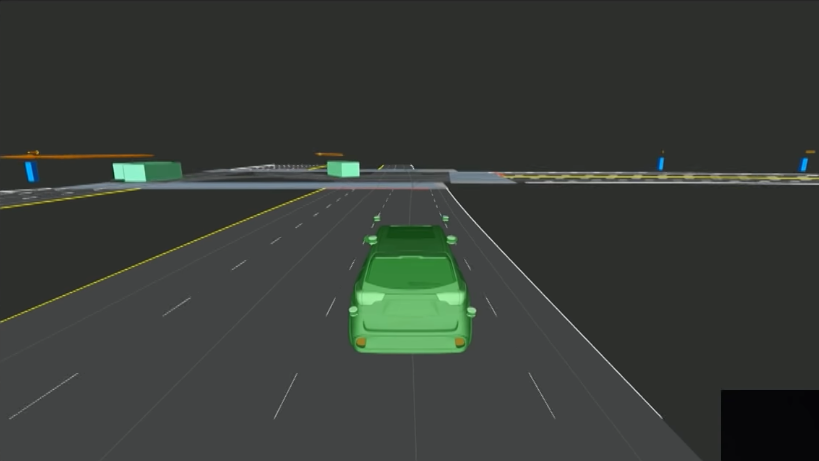
\includegraphics[width=0.8\textwidth]{images/zoox-siggraph-route-network.png}
     \end{center}
     \legend{Source: Adapted from \cite{zoox-unreal-siggraph-2017}.}
    \end{figure}
    
    \begin{figure}[H]
     \caption{\label{fig:zoox-simulation-monitoring}
Zoox simulation environment with route estimation}
     \begin{center}
        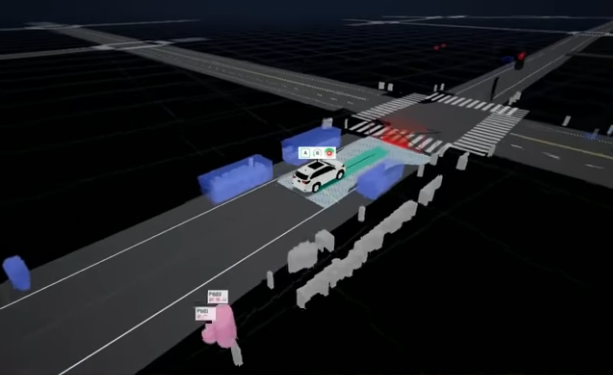
\includegraphics[width=0.8\textwidth]{images/zoox-simulation-monitoring.png}
     \end{center}
     \legend{Source: Adapted from \cite{zoox-fully-autonomous-driving}.}
    \end{figure}
    
    The current work relates to Zoox as both has as goal to provide visualization of autonomous vehicles algorithms. However, the cited startup considers more sensors (Velodyne, LiDAR) than our proposal (two stereo cameras) while also not necessarily focusing on performance for constrained systems.

\subsection{Image Segmentation and Depth}

    One of the major problems in the 3D environment reconstruction and computational vision is to develop a system capable of accurately discriminating each of the elements present in the environment.
    
    For the semantic association problem, \cite{semantic_article} proposes the use of deep convolutional networks in contrast to volumetric approaches operating directly on surface geometry. Crucially, the construction is applicable to unstructured point clouds and other noisy real-world data. The results can be seen in \autoref{fig:semantic-tangent-cnn}.

    \begin{figure}[H]
     \caption{\label{fig:semantic-tangent-cnn}
Top: point cloud from the Semantic3D dataset. Bottom: semantic segmentation produced by the approach.}
     \begin{center}
        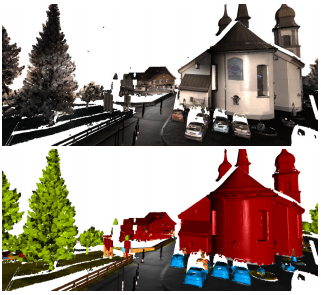
\includegraphics[width=0.5\textwidth]{images/depth_convul.png}
     \end{center}
     \legend{Source: Adapted from \cite{semantic_article}.}
    \end{figure}
    
    The current work relates to \cite{semantic_article} by having point clouds as input. However, while \cite{semantic_article} associate semantic meaning to data, our work have as input semantic images obtained by the current autonomous-driving algorithm in the environment.
    
    Aside from a semantic approach, to accurately discriminate elements in a scene for a virtual representation, it's important to estimate the distance and position of elements. \cite{toyota-depth} is an example of work that tries to improve the state of art on depth estimation (results shown in \autoref{fig:depth-superdepth}).

    \begin{figure}[H]
     \caption{\label{fig:depth-superdepth}Trained Monocular
disparity estimation network in a self-supervised manner
using a synchronized stream of stereo imagery, relieving
the need for ground truth depth labels}
     \begin{center}
        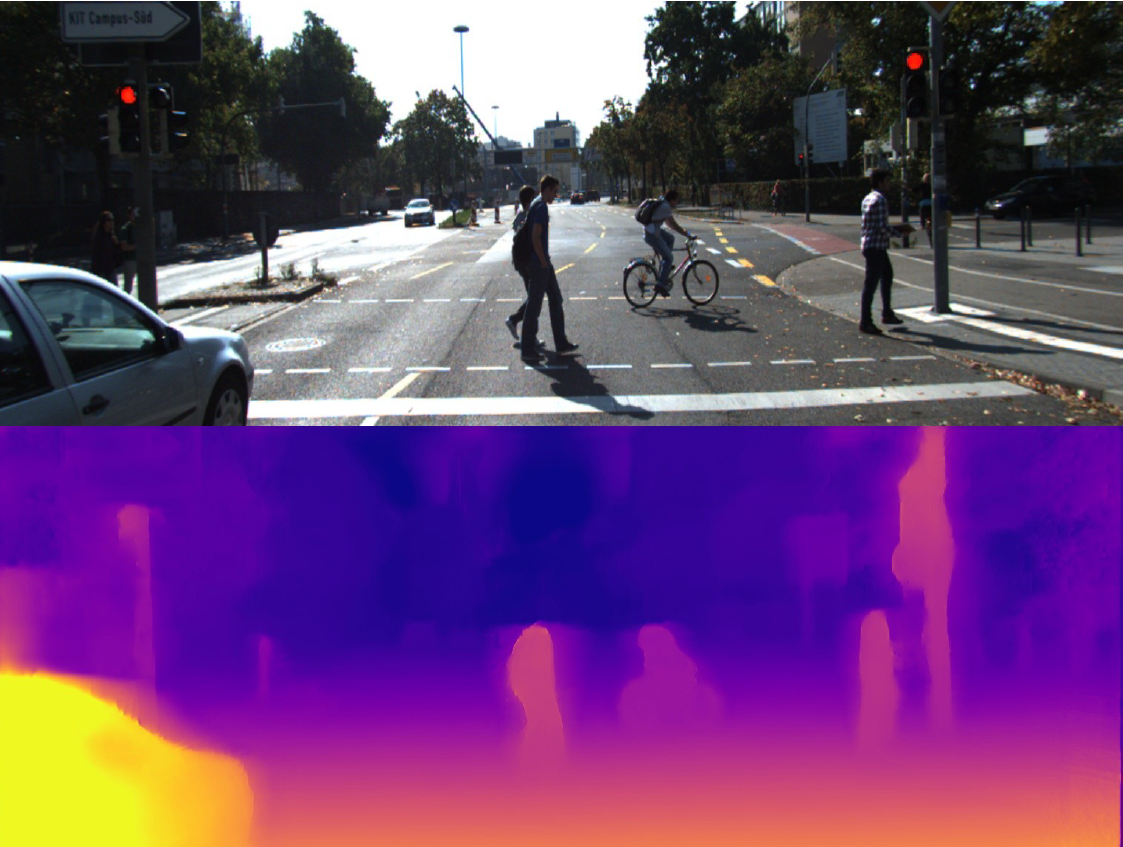
\includegraphics[width=0.45\textwidth]{images/superdepth-toyota.PNG}
     \end{center}
     \legend{Source: \cite{toyota-depth}}
    \end{figure}

    The current work doesn't focus on the creation of a new depth estimation method, as this topic deserves a research of its own. However, on the proposed system depth calculation is part of the pipeline, and a method for it will be explored on the development section.

\subsection{CARLA: An Open Urban Driving Simulation}

    According to CARLA's Website \cite{carla-official-website}, it's a simulator developed from the ground up to support development, training, and validation of autonomous urban driving systems. A open-source project that provides open digital assets (urban layouts, buildings, vehicles) that were created for this purpose and can be used freely. It is a complex simulator platform that supports flexible specification of sensor suites and environmental conditions (such as in \autoref{fig:carla_urban_environment}). In this platform it's possible to test a several kind of system that needs a urban environment. In addition, the system can generate performance reports.
    
    \begin{figure}[H]
     \caption{\label{fig:carla_urban_environment}
A street in Town 2, shown from a third-person view in four weather conditions. Clockwise from top left: clear day, daytime rain, daytime shortly after rain, and clear sunset.}
     \begin{center}
        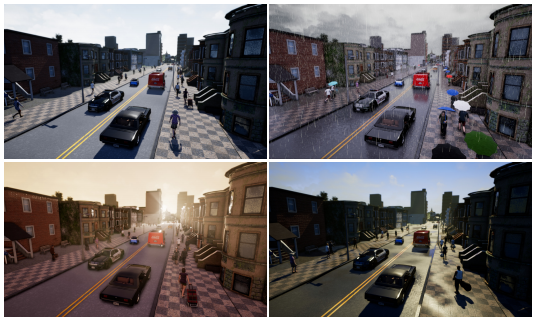
\includegraphics[width=0.8\textwidth]{images/urban_environment.png}
     \end{center}
     \legend{Source: Adapted from \cite{Dosovitskiy17}.}
    \end{figure}
    
    The simulator engine is defined primarily in the paper \cite{Dosovitskiy17} as the development of the environment and sensors. The environment, as shown in \autoref{fig:carla_urban_environment}, is composed of 3D models of static objects such as buildings, vegetation, traffic signs, and infrastructure, as well as dynamic objects such as vehicles and pedestrians. And then the authors used the following steps to build urban environments: (a) laying out roads and sidewalks; (b) manually placing houses, vegetation, terrain, and traffic infrastructure; and (c) specifying locations where dynamic objects can appear (spawn).
    
    About the sensors, CARLA allows for flexible configuration of the agent’s sensor suite. At the time of writing, sensors are limited to RGB cameras and to pseudo-sensors that provide ground-truth depth and semantic segmentation, such as \autoref{fig:carla_sensors}.
    
     \begin{figure}[H]
     \caption{\label{fig:carla_sensors}
Three of the sensing modalities provided by CARLA. From left to right: normal vision camera, ground-truth depth, and ground-truth semantic segmentation. Depth and semantic segmentation are pseudo-sensors that support experiments that control for the role of perception. Additional sensor models can be plugged in via the API.}
     \begin{center}
        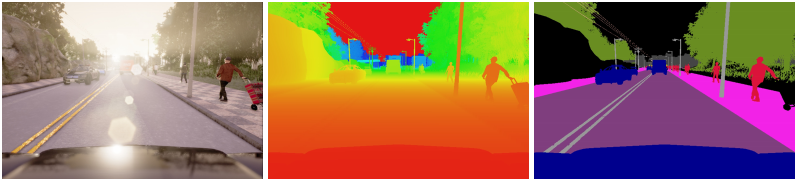
\includegraphics[width=0.8\textwidth]{images/sensor_carla.png}
     \end{center}
     \legend{Source: Adapted from \cite{Dosovitskiy17}.}
    \end{figure} 

    The sensors are be able to segmented 12 semantic classes: road, lane-marking, traffic sign, sidewalk, fence, pole, wall, building, vegetation, vehicle, pedestrian, and other. Therefore, CARLA manages not only to create a realist urban environment, but also to provide tools that allow the complete analysis of the environment around the car.
    
    The current work relates to CARLA as both proposes software with the use of computer graphics to assist the field of autonomous driving. However, CARLA's provides a virtual environment to test autonomous driving algorithms and compare them, while this research is focused in representing an approximation of the environment surrounding a real autonomous car and considering constraints of the real-world (as intrinsic sensor noise and computational limitation).

\section{Point Cloud Generation}

    This section contains concepts utilized to generate point cloud of a scene, and from it extract entity information by feature extraction methods. Point clouds generation steps are separated as camera calibration; disparity and semantic images generation and point cloud creation. These steps can be conceptual defined as the \autoref{fig:conceptual_flow} shows. 
    
        \begin{figure}[H]
     \caption{\label{fig:conceptual_flow}
Conceptual Flow to Generate a Point Cloud}
     \begin{center}
        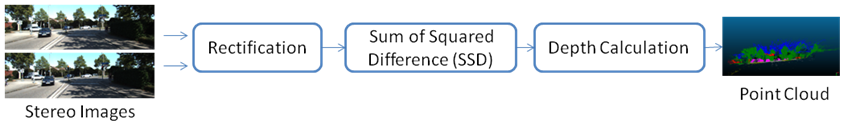
\includegraphics[width=1\textwidth]{images/conceitual_flow.png}
     \end{center}
     \legend{Source: Authors of this study.}
    \end{figure}
    
    As in \autoref{fig:conceptual_flow} flow, one must first calibrate the system according to the camera configuration used by conducting image rectification. Next, the Sum of Square Difference (SSD) calculation is used to obtain the disparity map and then calculate the depth of each scene element. The following subsections explain each of these steps in detail.
    
\subsection{Camera Calibration}

    Cameras have a natural distortion due to physics constraints and different types of lens. The more common are the Barrel and Pincushion distortions, and, according to \cite[p.1]{Vass2003ApplyingAR} “The first is due to the fact that many wide angle lenses have higher magnification in the image center than at the periphery. This causes the image edges to shrink around the center and form a shape of a barrel”. On the other hand, the Pincushion has the opposite effect, causing many wide angle lenses to have high magnification in the periphery of the image. Both are shown in \autoref{fig:lens-distortion}. It’s important to calibrate the cameras in order to eliminate these distortions as much as possible. 
    
    \begin{figure}[H]
     \caption{\label{fig:lens-distortion}
Types of radial distortion (a) Ideal image with no distortion, (b) Barrel Distortion, (c) Pincushion Distortion.}
     \begin{center}
        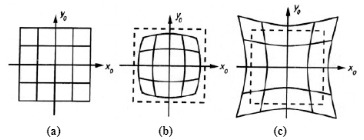
\includegraphics[width=0.7\textwidth]{images/lens.png}
     \end{center}
     \legend{Source: \cite{lensRef}.}
    \end{figure}    
    
    In addition to distortion, calibration is also important for obtaining intrinsic parameters. According to \cite{cameraCalibration1}, "the intrinsic parameters serve to relate the pixel coordinates relative to the images with the coordinates of points of space measured in the referential system originating in the center of the chamber. These parameters depend exclusively on the physical characteristics of the camera (its internal geometry, lens type) ". \cite{cameraCalibration2}, in a laboratory report, shows the main intrinsic parameters to be observed: Focal Distance, Optical Center of the image, Coefficient of lag, and, of course, distortions.

    The focal length, in pixels, represents the distance between the projection center and the image plane; The optical center represents the coordinates of the optical center of the image in frame memory; The lag coefficient represents the angle between the x-axis, y-axis, z-axis of the image in frame memory and the distortions representing the radial and tangential distortion coefficients.
    
    This research uses the distortions parameters, camera matrix and dataset with street pictures publicly available \cite{Geiger2013IJRR}.

\subsection{Epipolar Geometry}

    Epipolar Geometry refers to a mathematical operation that indicates how far apart the components of a scene are. With the help of two cameras (stereo cameras) it is possible to cross similar points of the same image and trace their spatial differences.

    To understand the concept of epipolar geometry, it is necessary to understand the line of projection. Considering an image of any scene, as shown in \autoref{fig:epipolar00}, it can be said that the projection line is the black line that cuts perpendicularly the image. In addition, for understanding, it is necessary to consider \(O_{1}\) the plane that the camera is and \(U_{1}\) the plane that shows the scene of the image.
    
    \begin{figure}[H]
     \caption{\label{fig:epipolar00}
Projection Line}
     \begin{center}
        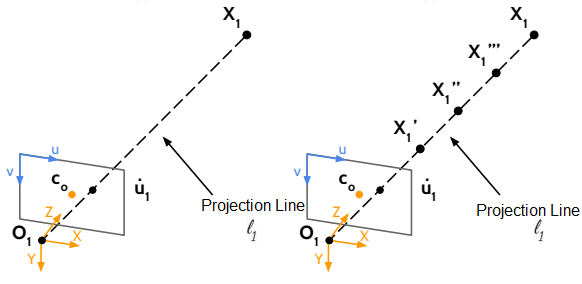
\includegraphics[width=0.5\textwidth]{images/epipolar0.png}
     \end{center}
     \legend{Source: Adapted from \cite{geometriaEpipolarLeonardo}.}
    \end{figure}

    It can be noted by looking at the image that any object located above the projection line (represented by \(X^{'}\), \(X^{''}\) and \(X^{'''}\)) will be superimposed (or hidden). The disparity matrix serves precisely to understand, from images, the depth of this projection line. And for this, a second camera is used, as shown in \autoref{fig:epipolar01}.

    \begin{figure}[H]
     \caption{\label{fig:epipolar01}
Triangulation of a point}
     \begin{center}
        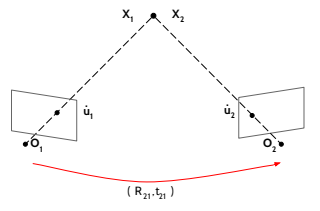
\includegraphics[width=0.5\textwidth]{images/epipolar1.png}
     \end{center}
     \legend{Source: \cite{geometriaEpipolarLeonardo}.}
    \end{figure}
    
    It is possible to see the projection line using a second camera. Therefore it's also possible to match common points between these images, such as in \autoref{fig:epipolar02}.

    \begin{figure}[H]
     \caption{\label{fig:epipolar02}
Matching Points}
     \begin{center}
        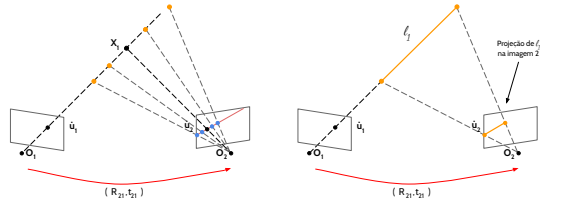
\includegraphics[width=0.7\textwidth]{images/epipolar2.png}
     \end{center}
     \legend{Source: \cite{geometriaEpipolarLeonardo}.}
    \end{figure}
    
    By treating the two images, eliminating their distortions and rectifying one against the other, it is possible to obtain something called the "Baseline" \cite{geometriaEpipolarLeonardo}, shown in \autoref{fig:epipolar03}.

    \begin{figure}[H]
     \caption{\label{fig:epipolar03}
Baseline}
     \begin{center}
        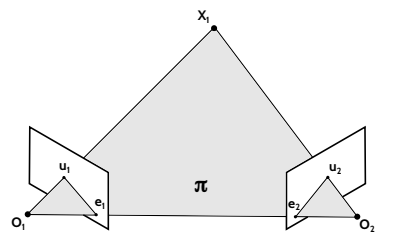
\includegraphics[width=0.5\textwidth]{images/epipolar3.png}
     \end{center}
     \legend{Source: \cite{geometriaEpipolarLeonardo}.}
    \end{figure}
    
    In his thesis \cite{geometriaEpipolarLeonardo} explain that with this configuration it's possible to define a \(\pi\) plane.
    
    The point \(e_{1}\), called the epipolo, is a projection of the optical center of the camera 2 (\(O_{2}\)) in the plane of the image of the camera 1. The epipolo \(e_{2}\) is found in the same way. The line is formed by points \(O_{1}\) and \(O_{2}\), where it connects the optical centers of the cameras is called the baseline. Its intersection with the planes of the images form epipolar lines. 
    
\subsection{Disparity and Sum of Squared Difference}

    Disparity matrix is a set containing the x-axis distance differences from two pixels obtained from left and right images. This matrix can be acquired from the pixels similarity (such as \autoref{fig:similaridade}) and Sum of Squared Difference (SSD) calculation, in code it can be obtained by a class called StereoSGBM using the OpenCV framework \cite{openCVCalibration}. This class match the analyzed function from two inputs: the left and right rectified pictures of the same scene, with requirement of having the images in grayscale.
    
    \begin{figure}[H]
     \caption{\label{fig:similaridade}
Camera Stereo configuration and Similarity of pixel}
     \begin{center}
        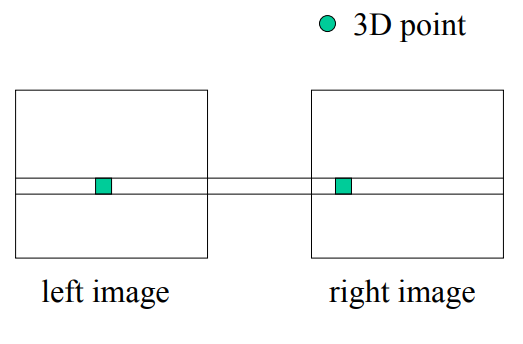
\includegraphics[width=0.5\textwidth]{images/similaridade.png}
     \end{center}
     \legend{Source: \cite{SSD_teste}.}
    \end{figure}
    
    According to the \autoref{fig:similaridade}, the point matching is performed when a common point is found in the two images and the SSD calculation is responsible to find this common pixel. This calculation can be defined by the following equation:
    
    \begin{center}
        \begin{equation}\label{eq:disparidade}
        C_{r}(x, y, d) = \sum_{(u,v)\epsilon W_{m}(x,y)}[I_{l}(u,v)-I_{r}(u-d, v)]^{2}
        \end{equation}
    \end{center}
    
    From the moment images are rectified, it can be stated that: given a horizontal pixel row in an image, there will be a corresponding pixel row in the other image. The SSD calculation is responsible for analyzing pixels in a row and finding the most similar pixels between them. An approach to find the similarity between one pixel and another is to power of two the subtraction of these two pixels, as \autoref{eq:disparidade} shows. Where \(I_{l}\) is the left image; \(I_{r}\) is the right image; \(u\) and \(v\) pixel position coordinates; and \(d\) the variation in \(x\) of the pixel. \autoref{fig:epipolar04} exemplifies the calculation in a more visual manner.
    
    \begin{figure}[H]
     \caption{\label{fig:epipolar04}
SSD Calculation}
     \begin{center}
        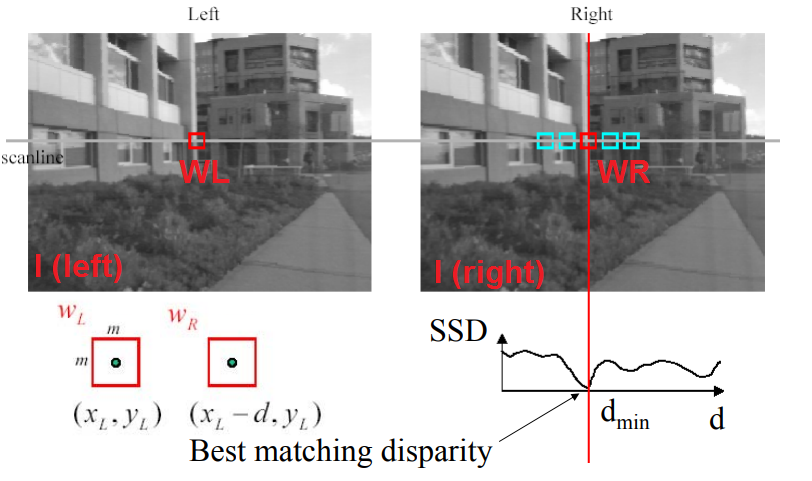
\includegraphics[width=0.9\textwidth]{images/matching_point.png}
     \end{center}
     \legend{Source: \cite{SSD_teste}.}
    \end{figure}
    
    The analysis is faithfully represented by \autoref{fig:epipolar04}, it is possible to observe how each step is performed: First, it defines which pixel should be analyzed in the first image; Next, the pixel row of the second image is defined as the first; Then, the SSD is calculated in the first pixel and its horizontal component varies in order to perform the same subtraction throughout the line; Lastly, it will have a vector of values that will represent which close each pixel of that line is in relation to the the first image pixel. The one with the lowest value will be the pixel most likely to match.
    
\subsection{Point Cloud}

    Point Cloud is a 3D reconstruction of a stereo photo, generated from a disparity map. The function used to do this on the OpenCV framework is called reprojectImageTo3D() and has an important output: A matrix containing x, y and z values with an intensity value in gray scale that shows the distance of each pixel (point) - The closer the camera is to the point, darker is the pixel.
    
    The reprojectImage3D function is an OpenCV feature used to become transparent the calculations and concepts used in the 3D scenario reconstruction. A calculation that uses as epipolar geometry principle and works two important concepts: disparity and depth. Using this geometry, the 3D problem become a 2D problem and thus, it's possible discuss about the disparity and depth concepts. \autoref{fig:epipolar05} evidence how these concepts are joined together for the reconstruction of a 3D scenario.

    \begin{figure}[H]
     \caption{\label{fig:epipolar05}
Disparity and Depth}
     \begin{center}
        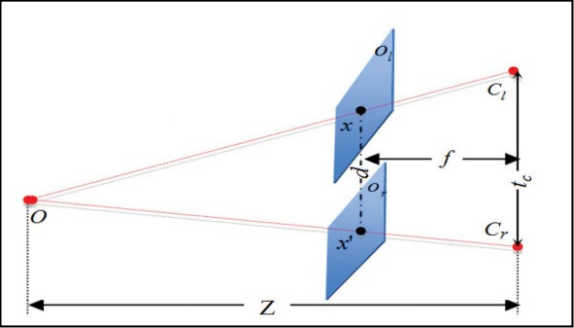
\includegraphics[width=0.8\textwidth]{images/mapaDisparidade.png}
     \end{center}
     \legend{Source: \cite{epipolarDispNat}.}
    \end{figure}
    
    In the image processing conception, it has as disparity the proximity of the same object described in the two images and it has as depth the actual distance of the object in relation to the two cameras.
    
    Similar to \autoref{fig:epipolar03}, it can be stated that once a baseline is defined, the 3D problem around the depth of the elements in the scene becomes two-dimensional similar triangles. Therefore, it can be said that the height of this triangle can be represented by \autoref{eq:profundidade}, since the base of the smaller triangle can be described by the disparity equation, as shown in \autoref{eq:disparidade}.    
    
    \begin{equation}\label{eq:profundidade}
    Z = \frac{t_{c}.f}{d}
    \end{equation}
    \begin{equation}\label{eq:disparidade}
    d = |x_{l}-x_{r}|
    \end{equation}

    Thus, it's possible to discover how deep is each pixel and print them in a 3D scenario. This scenario is called a point cloud.

    There are many applications with a point cloud in a 3D environment. It is usually used in conjunction with an algorithm to treat the surface of these points and reconstruct an approximate image from those points with graphic details. Thus, it's possible to reconstruct the real environment by a 3D environment with details. In the other hand, the point cloud can be used to acquire some useful data without a biggest graphic details, such as: size of different objects in scene, the center of mass, object directions and others.

    The \autoref{fig:point_cloud_ex} shows the point cloud and the possible applications with it. 
    
    \begin{figure}[H]
     \caption{\label{fig:point_cloud_ex}
Point cloud examples}
     \begin{center}
        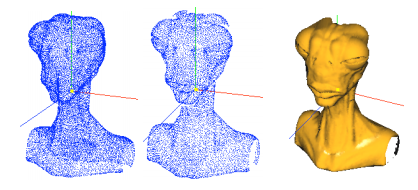
\includegraphics[width=0.8\textwidth]{images/imagem_point_cloud.png}
     \end{center}
     \legend{Source: \cite{pointCloud_ex}.}
    \end{figure}

In the first image, it can be noticed the pure point cloud – a 3D representation of a Alien with points. Alexandre, in his article \cite{pointCloud_ex}, used a reflection conception to describe the image graphically. In the other hand, it’s possible to discover information such as center of mass and substitute the point cloud to an alien's art.

\subsection{Semantic Context}

    A real image is made up of several objects and elements different from each other. In an urban environment, an image can contain pedestrians, cars, streets, animals, houses, poles and other elements that a human can easily differentiate. However, for an algorithm it is a complex task.

    In his thesis, Giovani \cite{giovaniThesis} describes a code capable of performing this objects differentiation in an urban image and compares the results obtained with other algorithms used in the literature. With its algorithm, it is able to discriminate road, sidewalk, vehicles, buildings, sky, vegetation and void spaces - spaces without discrimination.

    Giovani \cite{giovaniThesis} evidences the result of three approaches developed by him: ProbBoost, HistonBoost and ANN (Such as \autoref{fig:semanticaGi}). To use as a parameter and to train the neural network that will contribute to these approaches, the Ground Truth concept is used - an image that graphically represents the differentiation of the objects in the scene, as shown in \autoref{fig:semantic01}.

    \begin{figure}[H]
     \caption{\label{fig:semanticaGi}
Some results of Giovani's Thesis}
     \begin{center}
        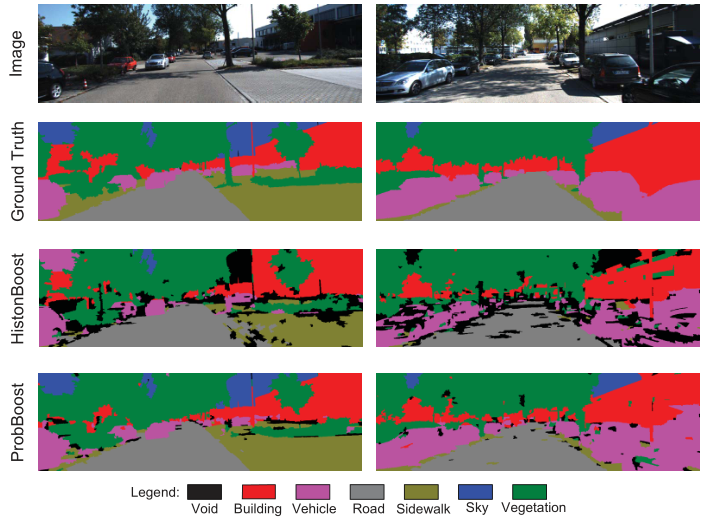
\includegraphics[width=1\textwidth]{images/semanticaGi.png}
     \end{center}
     \legend{Source: \cite{giovaniThesis}.}
    \end{figure}    

    \begin{figure}[H]
     \caption{\label{fig:semantic01}
Semantic Image}
     \begin{center}
        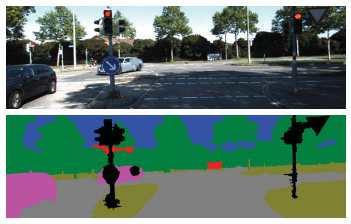
\includegraphics[width=0.7\textwidth]{images/semantic01.png}
     \end{center}
     \legend{Source: \cite{giovaniThesis}.}
    \end{figure}    
    
    In this project, the images generated in the Giovani's research \cite{giovaniThesis} named as Ground Truth are used as a semantic image. The urban environment images are analyzed with the help of the dataset provided by KITTI. KITTI's dataset is an urban image dataset created by Karlsruhe Institute of Technology (KIT).

\subsection{Difficulties}

    \cite{SSD_teste} in his lecture explain that this stereo reconstruction pipeline has some problems. Such as:
    
    \begin{itemize}
    \item Camera calibration errors;
    \item Poor image resolution;
    \item Occlusions;
    \item Violations of brightness constancy (specular reflections)
    \item  Large motions;
    \item Low-contrast image regions;
\end{itemize}

    All of these points are used for the analysis of results.
    
\section{Feature Extraction}

    This section approaches feature extraction methods for appliance on set of points with the final goal of describing entities on a scene. Since this project consider scene semantic information as input. Thus, there is exploration on methods for recognition of different categories. 
    
\subsection{Center of Mass}

    According to \cite[p. 219]{halliday-Mass-Center}, calculating the center of mass of 3D particles is possible by the following equation:
    
    \begin{equation}\label{eq:MassCenterX1}
    x_{mc} = \frac{1}{M}\sum_{i=1}^{n}m_{i}x_{i} 
    \end{equation}
    
    \begin{equation}\label{eq:MassCenterY1}
    y_{mc} = \frac{1}{M}\sum_{i=1}^{n}m_{i}y_{i}
    \end{equation}
    
    \begin{equation}\label{eq:MassCenterZ1}
    z_{mc} = \frac{1}{M}\sum_{i=1}^{n}m_{i}z_{i}
    \end{equation}
    
    Where \(m\) is the weight of the particle and \(M\) is the total weight of all particles together. In the case of a picture, all points have the same weight (value \(1\)) and \(M\) is equal to the total number of particles. Thus, this equation can be simplified to:
    
    \begin{equation}\label{eq:MassCenterX2}
    x_{mc} = \frac{1}{M}\sum_{i=1}^{n}x_{i} 
    \end{equation}
    
    \begin{equation}\label{eq:MassCenterY2}
    y_{mc} = \frac{1}{M}\sum_{i=1}^{n}y_{i}
    \end{equation}
    
    \begin{equation}\label{eq:MassCenterZ2}
    z_{mc} = \frac{1}{M}\sum_{i=1}^{n}z_{i}
    \end{equation}
    
    
\subsection{Box of lower and upper limits of the object}

    There are different ways of calculating limits for a object defined by a set of points. Two approached in this section are the use of center of mass \& geometric centroid, and the analysis tool of variance.

    The first method calculates the center of mass of an object, refer to it as origin, and for each direction calculates the geometric centroid of points, defining them as direction's limit. Repeating this procedure for all directions creates a box which represents the object's approximate size. This approach is not efficient for the reason that it will always set limits lower than the actual limit of the object. Because it is an average of points, this value will hardly match the maximum point of the object.

    On the other hand, \cite{estatistic-douglas} explain a more suitable way of finding these limits. The variance of a random variable is a measure of dispersion, or scatter, in the possible values for the variable. Thus, it's possible to find an approximate value of dispersion for the center of mass (\(\upsilon\)) using the variance formula in \autoref{eq:variance}.

    \begin{equation}\label{eq:variance}
    \sigma^{2} = \sum_{x}(x-\upsilon)^{2}f(x) 
    \end{equation}

    It's possible to find an approximate maximum point of different directions, and then create an upper and lower box of the object, when using \autoref{eq:variance}. Finally, the difference between the upper and lower limits is calculated in order to define the width, height and length values.


\section{3D software architecture}

    This section approaches 3D software architectures considering their motivations, pros \& cons, and implementations. As that one of this project goals is the development of a 3D environment using computer graphics.
    
\subsection{Software Architectures in the industry}

    When considering reference sources for software architectures (especially for 3D and simulation software) the industry related work, e.g. \cite{leonard-thief-postmortem}, stands out as the content theme doesn't appeal strongly to academic environment due to the evident product focused approach instead of theoretical.
    
    Software architecture design choice has direct impact on the performance, as explored in \cite{albrecht-pitfalls-OOP-GCAP09}. Albrecht presented in GCAP 2009 a performance comparison of different data designs implementations. 
    
    The test scene tree consists of an object class containing general data (Object), class to render object (Drawable & Cube), class to update geometrical transforms (Modifier), and container class which store access to objects (Node). The standard data for comparison is shown in \autoref{fig:albrecht-simple-oo-scene-tree}. 
    
    \begin{figure}[H]
        \caption{
        \label{fig:albrecht-simple-oo-scene-tree}
            Simple Scene Tree
        }
        \begin{center}
        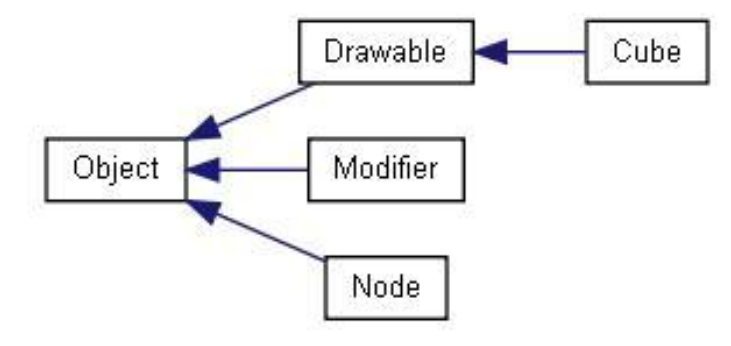
\includegraphics[width=0.5\textwidth]{images/albrecht-simple-oo-scene-tree.png}
        \end{center}
        \legend{Source: Adapted from \cite{albrecht-pitfalls-OOP-GCAP09}.}
    \end{figure}    
    
    The test execution for data in the scene corresponds of:
    
    \begin{itemize}
        \item 11,111 nodes/objects in a tree 5 levels deep
        \item Every node being transformed
        \item Hierarchical culling of tree
        \item Render method being empty
    \end{itemize}
    
    The different data organizations approaches iterate on the previous, and consisting of:
    
    \begin{itemize}
        \item Simple Object Oriented following the Scene tree organization
        \item Contiguous data allocation with use of homogeneous sequential sets
        \item Flat design by removing hierarchy of calls
        \item Flat design with prefetching due to predictable data accesses
    \end{itemize}
    
    Albrecht then presents the final test results for different data designs, shown in \autoref{fig:albrecht-cache-impact}. The most considerable performance gains were obtained by the continuous allocation of data (less encapsulation) and the flattening of hierarchy (less layers of abstraction).  
    
    \begin{figure}[H]
        \caption{
        \label{fig:albrecht-cache-impact}
            Cache impact of different data design approaches (values in milliseconds).
        }
        \begin{center}
        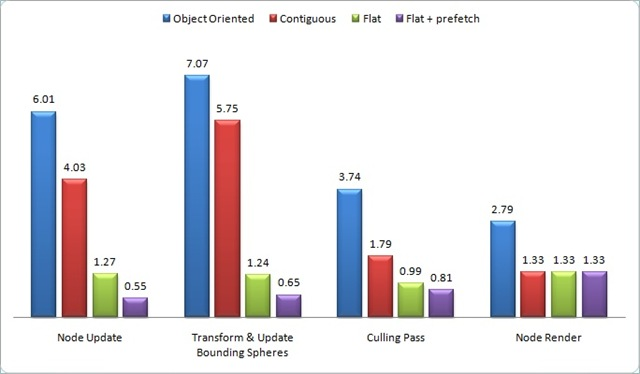
\includegraphics[width=0.8\textwidth]{images/albrecht-cache-impact.jpg}
        \end{center}
        \legend{Source: Adapted from \cite{albrecht-pitfalls-OOP-GCAP09}.}
    \end{figure}
    
    By the previous shown study its evident that to obtain better performance what have to be explored is the way data is accessed and stored. This design approach is justified by the Processor-Memory Gap explored in the next subsection.

\subsection{Processor-Memory Gap}
    
    The Processor-Memory Gap is described by the difference in time between processor memory request and the latency of DRAM access. It describes a problem where the processor performance improved in higher rate than the memory performance improved \cite{computer-architecture-a-quantitative-approach-6ed}. \autoref{fig:performance-gap-processor-memory} shows that the gap increased over many years but is currently in a slowdown due to the lack of improvements in single processors. Although \autoref{fig:performance-gap-processor-memory} shows values for single core processors, the number of multiple cores in processors implies growth of the gap due to the demand of DRAM bandwidth as the number of cores grows.
    
    \begin{figure}[H]
        \caption{
        \label{fig:performance-gap-processor-memory}
            Single processor performance projections against the historical performance improvement in time to access main memory (Processor line shows the increase in memory requests per second on average. Memory line shows the increase in DRAM accesses per second).
        }
        \begin{center}
        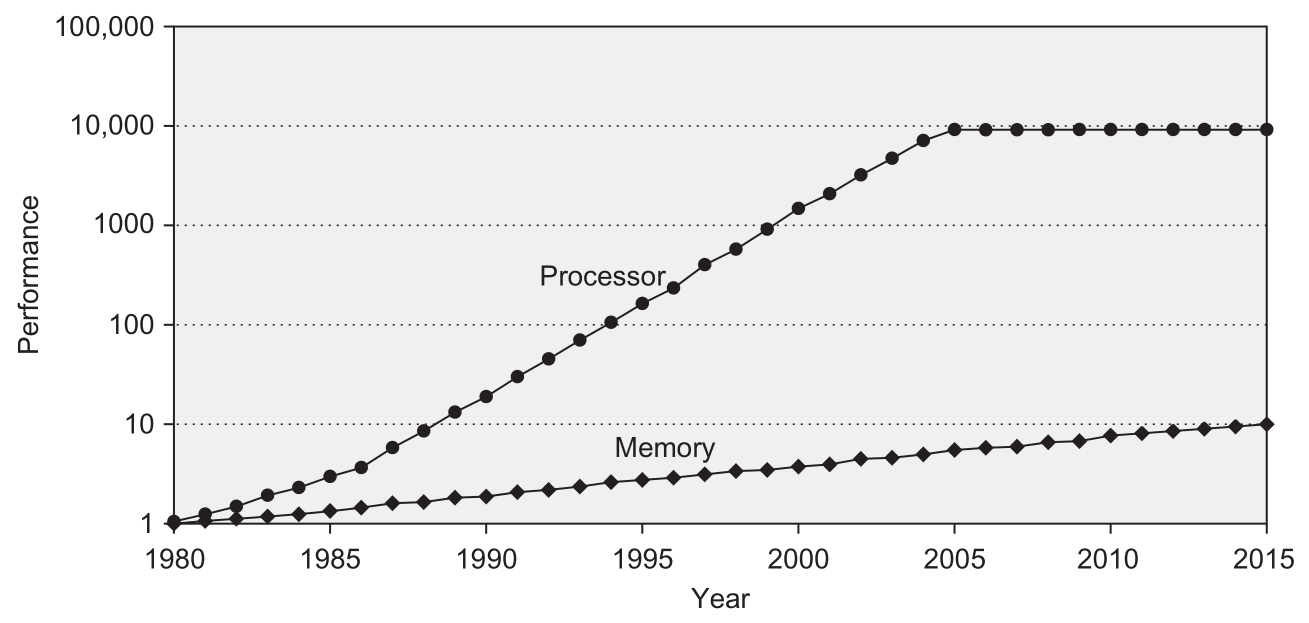
\includegraphics[width=1\textwidth]{images/performance-gap-processor-memory.png}
        \end{center}
        \legend{Source: \cite{computer-architecture-a-quantitative-approach-6ed}.}
    \end{figure}

    As this problem doesn't have an expected hardware solution, it ends up being the software layer job to work with the implied handicap when it appears as an obstacle for an application. In the next subsection we approach Data-Oriented Design, a pattern of software development that is less affect by the Processor-Memory gap problem as the number of memory accesses and cache misses tends to be reduced.
    
\subsection{Entity Component Systems and Data-Oriented Design}

    Entity Component Systems (ECS) is an architectural pattern for software development. There is no concrete definition on its architecture scope, but it does often share Data-Oriented Design (DOD) techniques which focus on designing for performance \cite{llopis-game-engine-gems-2}.
    
    This architecture approach is better suited, for applications such as Game Engines or Real-Time Simulators, which are highly demanding processing software requiring constant main memory access to run in real-time. 
    
    Good case results of implementations for the ECS concept on the industry goes back decades \cite{leonard-thief-postmortem} accompanied by the increased storage of data and the demand of its processing on applications. However, implementation efforts on ECS are still relevant, being focus of features for powerful software \cite{johansson-ecs-unity-gdc-2018}.

    DOD main focus can be considered to be cache coherency. In consequence of this pursue the architecture of code generated by it tends to be decoupled and simple in scope, due to not having a world-approximation as Oriented-Programming encourages. 
    
    As a mean to characterize Data-Oriented Design, \cite{llopis-game-engine-gems-2} consider its benefits and disadvantages. On \autoref{table:dod-benefits} his discourse for each aspect of DOD are listed and simplified.

    \begin{table}[H]
    \centering
    \caption{
        Data oriented design benefits \cite{llopis-game-engine-gems-2}, adaptation as table by Authors of this study.
    }
    \label{table:dod-benefits}
    \begin{tabular}{cc}\toprule
    \textbf{Benefits}                   & \textbf{Description} \\ \bottomrule \\
    Cache utilization                   & \begin{tabular}[c]{@{}l@{}} 
                                        Organization of data into large sequential\\
                                        blocks of homogeneous memory, processing\\ 
                                        it by running the same code on all its\\ elements.\end{tabular}
                                        \\\\ \hline \\
    Parallelization                     & \begin{tabular}[c]{@{}l@{}} 
                                        As we work from the data point of view, it\\ 
                                        becomes a lot easier to divide work up into\\ 
                                        parts that different cores can processes\\ 
                                        simultaneously with minimal synchronization.\\ \end{tabular} \\\\ \hline \\
    Less code                           & \begin{tabular}[c]{@{}l@{}}
                                        Code that before was doing boring book-\\
                                        keeping, or getter/setters on objects,\\ 
                                        or even unnecessary abstractions,\\ 
                                        all go away.\end{tabular}
                                        \\ \\ \bottomrule
    \textbf{Disadvantages}              & \textbf{Description} \\ \bottomrule \\
    It's different                      & \begin{tabular}[c]{@{}l@{}}
                                        So far, data-oriented design isn’t taught\\ 
                                        in Computer Science curricula, \\  
                                        ... so it is foreign to most team members.
                                        \end{tabular} \\\\ \hline \\
    Harder to see the big picture       &  \begin{tabular}[c]{@{}l@{}}
                                        Because of the emphasis on data and on\\
                                        small functions that transform data, it\\
                                        might be harder to see and express the\\
                                        big picture of the program [...]
                                        \end{tabular} \\\\ \bottomrule \\
    \end{tabular}
    \end{table}
    
    A better grasp on the idea of DOD can be obtained with code examples. Consider the two following implementations in C++ \cite{dice-data-oriented-design}. 
    
    \begin{itemize}
        \item \autoref{fig:dice_exampleOOP} uses Object-Oriented Programming and has the idea of creating a class Bot which stores data (attributes) and functionalities (methods);
        \item \autoref{fig:dice_exampleDOP} conforms to the Data-Oriented Design and has as focus generating the output data (in this case the "aiming direction"), doing that with a function which receives the input to be transformed.
    \end{itemize}
     
    \begin{figure}[H]
        \caption{
        \label{fig:dice_exampleOOP}
            Object-Oriented Programming code example
        }
        \begin{center}
        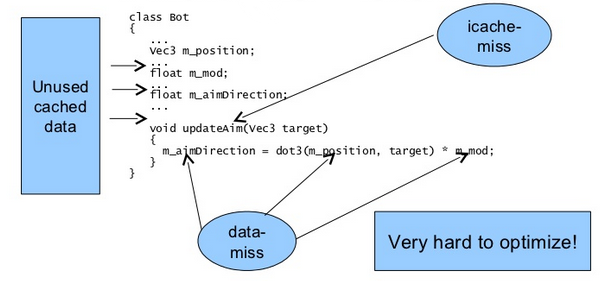
\includegraphics[scale=0.9]{images/dice-exampleOOP_Introduction-to-Data-Oriented-Design.png}
        \end{center}
        \legend{Source: \cite{dice-data-oriented-design}.}
    \end{figure}
    
    \begin{figure}[H]
        \caption{
        \label{fig:dice_exampleDOP}
            Data-Oriented Programming code example
        }
        \begin{center}
        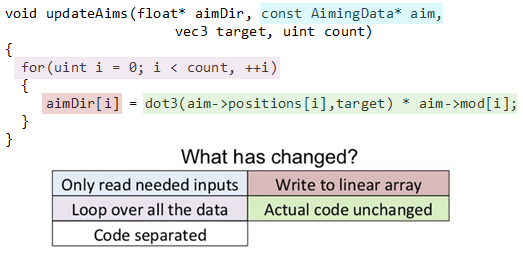
\includegraphics[scale=1]{images/dice-exampleDOP_Introduction-to-Data-Oriented-Design.png}
        \end{center}
        \legend{Source: Adapted from \cite{dice-data-oriented-design}.}
    \end{figure}
    
    It is possible to better visualize the descriptions made in \autoref{table:dod-benefits}, by comparing the two previous implementations. Instead of trying to represent the problem and its elements using known items from the real world as OOP did, DOD focus on solving the problem in its most simpler iteration.
    
    Considering previous data knowledge, as it is likely that there is more than one Bot and that "updateAims" will be called more than once, DOD optimizes memory requests by receiving as parameters the necessary input for processing (aligning it in cache) and doing the same operation for each cell of the "Bots" linear array. Thus eliminating cache misses and decoupling the code.
    
    In conclusion, comparing DOP with the well spread Object-Oriented Programming (OOP), DOP implies the requirement of engineers to know their data, and that structure and code refactoring is continuously present during DOP development to eliminate bottlenecks \cite{albrecht-latency-elephant}.



%%%%%%%%%%%%%%%%%%%%%%%%%%%%%%%%%%%%%%%%%%%%%%%%%%%%%%%%%%%%%%%%%%%%%%%%%%%%%%%%%%%%%%%%%%%%%%%%%%%%%%%%%%%%%%%%%%
